%!TEX encoding = UTF-8 Unicode
%!TEX root = ../lect-week01.tex

%%%%%%%%%%%%%%%%%%%%%%%%%%%%%%%%%%%%%%
\Subsection{Om programmering}

%%%

\begin{Slide}{Vad är programmering?}
\begin{itemize}
\item Programmering innebär att ge instruktioner till en maskin.
\item Ett \Emph{programmeringsspråk} används av människor för att skriva \Emph{källkod} som kan översättas av en \Emph{kompilator} till \Emph{maskinspråk} som i sin tur \Emph{exekveras} av en dator.
\end{itemize}


\begin{minipage}{.8\textwidth}
\begin{itemize}
\item Ada Lovelace skrev det första programmet redan på 1800-talet ämnat för en kugghjulsdator. 
\item Ha picknick i Ada Lovelace-parken på Brunnshög!
\end{itemize}
\end{minipage}%
\begin{minipage}{.2\textwidth}
\centering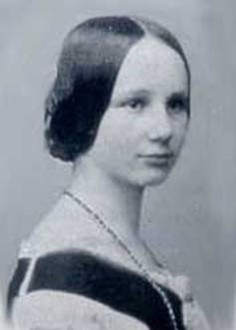
\includegraphics[width=0.6\columnwidth]{../img/ada}
\end{minipage}%
\begin{itemize}
\item \href{https://sv.wikipedia.org/wiki/Programmering}{sv.wikipedia.org/wiki/Programmering}
\item \href{https://en.wikipedia.org/wiki/Computer\_programming}{en.wikipedia.org/wiki/Computer\_programming}
\item \href{http://kartor.lund.se/wiki/lundanamn/index.php/Ada_Lovelace-parken}{kartor.lund.se/wiki/lundanamn/index.php/Ada\_Lovelace-parken}
\end{itemize}
\end{Slide}


\begin{Slide}{Vad är en kompilator?}
\begin{multicols}{2}
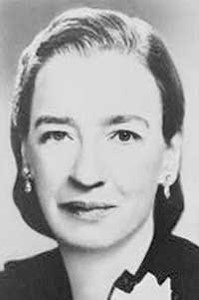
\includegraphics[width=0.8\columnwidth]{../img/grace}

\columnbreak %---------

Grace Hopper uppfann första kompilatorn 1952.\\
\href{https://en.wikipedia.org/wiki/Grace\_Hopper}{\small en.wikipedia.org/wiki/Grace\_Hopper}
\vskip1em
%https://www.sharelatex.com/blog/2013/08/29/tikz-series-pt3.html
\begin{tikzpicture}[node distance=1.8cm]
\node (input) [startstop] {Källkod};
\node(inptext) [right of=input, text width=2cm, scale=0.8,xshift=1.0cm]{För\\människor};
\node (compile) [process, below of=input] {Kompilator};
\node (output) [startstop, below of=compile] {Maskinkod};
\node(outtext) [right of=output, text width=2cm, scale=0.8,xshift=1.0cm]{För\\maskiner};
\draw [arrow] (input) -- (compile);
\draw [arrow] (compile) -- (output);
\end{tikzpicture}
\end{multicols}
\end{Slide}


\begin{Slide}{Vad består ett program av?}
\begin{itemize}
\item Text som följer entydiga språkregler (gramatik): 
\begin{itemize}
\item \Emph{Syntax}: textens konkreta utseende 
\item \Emph{Semantik}: textens betydelse (vad maskinen gör/beräknar)
\end{itemize}
\item \Emph{Nyckelord}: ord med speciell betydelse, t.ex. \code{if}, \code{else}
\item \Emph{Deklarationer}: definitioner av nya ord: \code{def gurka = 42}
\item \Emph{Satser} är instruktioner som \emph{gör} något: \code{print("hej")} 
\item \Emph{Uttryck} är instruktioner som beräknar ett \emph{resultat}: \code{1 + 1}
\item \Emph{Data} är information som behandlas: t.ex. heltalet \code{42}
\item Instruktioner ordnas i kodstrukturer: (SARA)
\begin{itemize}
\item \Emph{Sekvens}: ordningen spelar roll för vad som händer
\item \Emph{Alternativ}: olika saker händer beroende på uttrycks värde
\item \Emph{Repetition}: satser upprepas många gånger
\item \Emph{Abstraktion}: nya byggblock skapas för att återanvändas
\end{itemize}
\end{itemize}
\end{Slide}

\begin{Slide}{Exempel på programmeringsspråk}
Det finns massor med olika språk och det kommer ständigt nya. 
\vspace{1em}
\begin{multicols}{2}
Exempel:
\begin{itemize}
\item Java
\item C
\item C++
\item C\#
\item Python
\item JavaScript
\item Scala
\end{itemize}

\columnbreak %---------

Topplistor:
\begin{itemize}
\item \href{http://www.tiobe.com/index.php/content/paperinfo/tpci/index.html}{TIOBE Index}
\item \href{http://pypl.github.io/PYPL.html}{PYPL Index}
\end{itemize}
\vspace{1em}

\includegraphics[width=0.8\columnwidth]{../img/pypl}
\end{multicols}

\end{Slide}

\begin{Slide}{Varför Scala + Java som förstaspråk?}
\begin{itemize}
\item Varför Scala?
\begin{itemize}
\item Enkel och enhetlig syntax => lätt att skriva
\item Enkel och enhetlig semantik => lätt att fatta 
\item Kombinerar flera angreppsätt => lätt att visa olika lösningar
\item Statisk typning + typhärledning =>  färre buggar + koncis kod
\item Scala Read-Evaluate-Print-Loop => lätt att experimentera
\end{itemize}

\item Varför Java?
\begin{itemize}
\item Det mest spridda språket
\item Massor av fritt tillgängliga kodbibliotek
\item Kompabilitet: fungerar på många platformar
\item Effektivitet: avancerad \& mogen teknik ger snabba program
\end{itemize}
\item Java och Scala fungerar utmärkt tillsammans
\item Illustrera likheter och skillnader mellan olika språk \\ => Djupare lärande
\end{itemize}
\end{Slide}

\begin{Slide}{Hello world}

\begin{REPLnonum}
scala> println("Hello World!")
Hello World!
\end{REPLnonum}

\begin{Code}
// this is Scala 

object Hello {
  def main(args: Array[String]): Unit = {
    println("Hejsan scala-appen!")
  }
}
\end{Code}


\begin{Code}[language=Java]
// this is Java 

public class Hi {
    public static void main(String[] args) {
        System.out.println("Hejsan Java-appen!");
    }
}
\end{Code}

\end{Slide}

\begin{Slide}{Utvecklingscykeln}
editera; kompilera; hitta fel och förbättringar; editera; kompilera; hitta fel och förbättringar; editera; kompilera; hitta fel och förbättringar; editera; kompilera; hitta fel och förbättringar; editera; kompilera; hitta fel och förbättringar; editera; kompilera; hitta fel och förbättringar; ...

\begin{Code}
upprepa(1000){
  editera
  kompilera
  testa
}
\end{Code}
\end{Slide}

\begin{Slide}{Utvecklingsverktyg}
\begin{itemize}
\item Din verktygskunskap är mycket viktig för din produktivitet. 
\item Lär dig kortkommandon för vanliga handgrep. 
\item Verktyg vi använder i kursen:
\begin{itemize}
\item Scala \Emph{REPL}: från övn 1
\item \Emph{Texteditor} för kod, t.ex \code{gedit}: från övn 2
\item Kompilera med \Emph{\code{scalac}} och \Emph{\code{javac}}: från övn 2
\item Integrerad utvecklingsmiljö (IDE)
\begin{itemize}
\item \Emph{Kojo}: från lab 1
\item \Emph{Eclipse} med plugin \Emph{ScalaIDE}: från lab 3
\end{itemize}
\item \Emph{jar} för att packa ihop och distribuera klassfiler
\item \Emph{javadoc} och \Emph{scaladoc} för dokumentation av kodbibliotek
\end{itemize}
\item Andra verktyg som är bra att lära sig:
\begin{itemize}
\item git för versionshantering
\item GitHub för kodlagring -- men \Alert{inte} av lösningar till labbar!
\end{itemize}
\end{itemize}
\end{Slide}


\ifkompendium\else  %%%%%%%%%%%%%%%%%%%%%%%%%%%%%%%%%%%%%%%%%%%%%%%%%

\begin{Slide}{Att skapa koden som styr världen}
\begin{multicols}{2}\footnotesize
I stort sett alla delar av samhället är beroende av programkod:
\begin{itemize}\scriptsize
\item kommunikation
\item transport
\item byggsektorn
\item statsförvaltning
\item finanssektorn
\item media \& underhållning
\item sjukvård
\item övervakning
\item integritet
\item upphovsrätt
\item miljö \& energi
\item sociala relationer
\item utbildning 
\item ...
\end{itemize}
\columnbreak %---------
Hur blir ditt framtida yrkesliv som systemutvecklare?
\begin{itemize}
\item  Redan nu är det en skriande brist på utvecklare och bristen blir bara värre och värre... \\
  \href{http://computersweden.idg.se/2.2683/1.634770/rekrytera-utvecklare}{CS 2015-08-17}
\item Störst brist är det på kvinnliga utvecklare: \\
\href{http://www.dn.se/ekonomi/it-branschen-hotas-av-brist-pa-kvinnor/}{DN 2015-04-02}
\item Global kompetensmarknad \\ 
  \href{http://computersweden.idg.se/2.2683/1.630901/det-finns-programmerare-och-sa-finns-det-programmerare}{CS 2015-06-14}\\
   \href{http://computersweden.idg.se/2.2683/1.634700/7-satt-att-bli-en-battre-programmerare}{CS 2015-08-15}
\end{itemize}
\end{multicols}
\end{Slide}

\begin{Slide}{Utveckling av mjukvara i praktiken}
\begin{itemize}
\item \Emph{Inte bara kodning:} kravbeslut, releaseplanering, design, test, versionshantering, kontinuerlig integration, driftsättning, återkoppling från dagens användare, ekonomi \& investering, gissa om morgondagens användare, ... 
\item \Emph{Teamwork:} Inte ensamma hjältar utan autonoma team i decentraliserade organisationer med innovationsuppdrag
\item \Emph{Snabbhet:} Att koda innebär att hela tiden uppfinna nya ''byggstenar'' som ökar organisationens förmåga att snabbt skapa värde med hjälp av mjukvara. Öppen källkod. Skapa kraftfulla API:er.
\item \Emph{Livslångt lärande:} Lär nytt och dela med dig hela tiden. Exempel på pedagogisk utmaning: hjälp andra förstå och använda ditt API $\implies$ \textit{Samarbetskultur}
\end{itemize}
\end{Slide}


\SlideImg{Programming unplugged: Två frivilliga?}{../img/unplugged}
\SlideImg{Editera och exekvera ett program}{../img/kojo}

\fi %%%%%%%%%%%%%%%%%%%%%%%%%%%%%%%%%%%%%%%%%%%%%%%%%%%%

\begin{Slide}{Literaler}
Literaler representerar ett fixt värde i koden. Literaler används för att skapa data i ett program.
\end{Slide}

\begin{Slide}{Uttryck}
Räknar ut något nytt baserat på existerande delar.
\end{Slide}

\begin{Slide}{Identifierare}
Namn på saker.
\end{Slide}

\begin{Slide}{Speciella identifierare}
Backticks för att komma runt krockar med nyckelord. \texttt{`var`}
\end{Slide}

%%%%%%%%%%%%%%%%%%%%%%%%%%%%%%%%%%%%%%
\ifkompendium\else
\Subsection{Meddelande från \href{http://lth.se/code}{Code@LTH}} 
\fi